\chapter{Küme Teorisi ve Fonksiyon Temelleri}

pytop'un tüm modülleri küme teorisi ve fonksiyon kavramları üzerine kuruludur.
Bu bölüm kılavuzun geri kalanında varsayılan ön koşulları pytop API'siyle pekiştirir.

%-------------------------------------------------------------------
\section{Konu}

\begin{definition}[Altküme ve Güç Kümesi]
$A \subseteq B \Longleftrightarrow \forall a \in A,\, a \in B$.
\textbf{Güç kümesi:} $\mathcal{P}(A) = \{S : S \subseteq A\}$,\quad
$|\mathcal{P}(A)| = 2^{|A|}$.
\end{definition}

İki kümenin işlemleri Venn şemasıyla görselleştirilir: $A\cup B$ üç bölgenin
tamamı, $A\cap B$ ortadaki örtüşen bölge, $A\setminus B$ ise $A$'nın $B$'den
ayrık kalan kısmıdır.

\begin{figure}[ht]
\centering
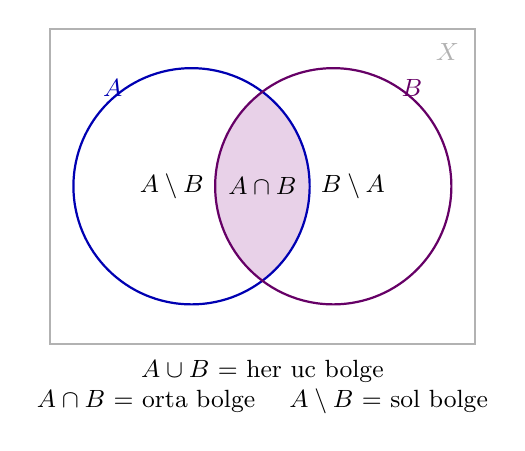
\begin{tikzpicture}[scale=1.0, font=\small]
  % evren kutusu
  \draw[gray!60, thick] (-2.7,-2.0) rectangle (2.7,2.0);
  \node[gray!60] at (2.35,1.7) {$X$};
  % A ve B daireleri (kesisim taranir)
  \begin{scope}
    \clip (-0.9,0) circle (1.5);
    \fill[violet!18] (0.9,0) circle (1.5);
  \end{scope}
  \draw[blue!70!black, thick] (-0.9,0) circle (1.5);
  \draw[violet!80!black, thick] (0.9,0) circle (1.5);
  \node[blue!70!black] at (-1.9,1.25) {$A$};
  \node[violet!80!black] at (1.9,1.25) {$B$};
  % bolgeler
  \node at (-1.15,0) {$A\setminus B$};
  \node at (0,0) {$A\cap B$};
  \node at (1.15,0) {$B\setminus A$};
  \node[align=center] at (0,-2.55)
    {$A\cup B$ = her uc bolge\\ $A\cap B$ = orta bolge \quad $A\setminus B$ = sol bolge};
\end{tikzpicture}

\caption{İki küme için $A\cup B$, $A\cap B$ ve $A\setminus B$ bölgeleri.}
\end{figure}

\begin{sezgi}
Tümleyen her zaman bir \textbf{evrene} ($X$) göre tanımlıdır; ``$A^c$'' tek
başına anlamsızdır. pytop bunu \texttt{complement(subset, universe)} imzasıyla
zorunlu kılar.
\end{sezgi}

\begin{karsiornek}
``$A\cup B$ her zaman $A$'dan büyüktür'' yanlıştır: $B\subseteq A$ ise
$A\cup B = A$. Örneğin $A=\{1,2,3\}$, $B=\{2\}$ için $|A\cup B|=|A|=3$.
\end{karsiornek}

\begin{definition}[Kartezyen Çarpım]
$A \times B = \{(a,b) : a\in A,\ b\in B\}$ ve $|A\times B| = |A|\cdot|B|$.
$A$ üzerinde bir bağıntı $R \subseteq A\times A$.
\end{definition}

\begin{figure}[ht]
\centering
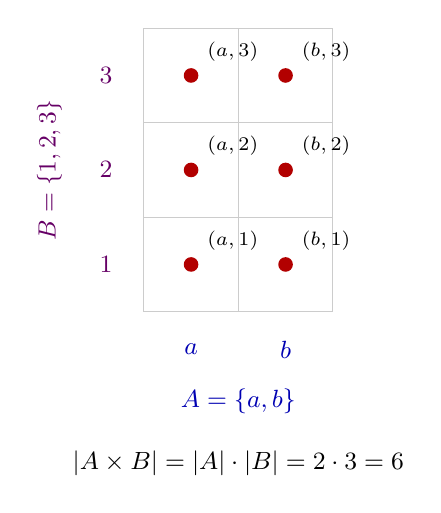
\begin{tikzpicture}[scale=1.2, font=\small]
  % 2 (yatay, A) x 3 (dikey, B) izgara
  \draw[gray!40] (0,0) grid (2,3);
  % A ekseni (yatay): a, b
  \node[blue!70!black] at (0.5,-0.4) {$a$};
  \node[blue!70!black] at (1.5,-0.4) {$b$};
  \node[blue!70!black] at (1.0,-0.95) {$A=\{a,b\}$};
  % B ekseni (dikey): 1, 2, 3
  \node[violet!80!black] at (-0.4,0.5) {$1$};
  \node[violet!80!black] at (-0.4,1.5) {$2$};
  \node[violet!80!black] at (-0.4,2.5) {$3$};
  \node[violet!80!black, rotate=90] at (-1.0,1.5) {$B=\{1,2,3\}$};
  % carpim noktalari (a,1)...(b,3)
  \foreach \x/\xl in {0.5/a, 1.5/b}
    \foreach \y/\yl in {0.5/1, 1.5/2, 2.5/3} {
      \fill[red!70!black] (\x,\y) circle (2.2pt);
      \node[anchor=south west, font=\scriptsize] at (\x+0.07,\y+0.05) {$(\xl,\yl)$};
    }
  \node at (1.0,-1.6) {$|A\times B| = |A|\cdot|B| = 2\cdot 3 = 6$};
\end{tikzpicture}

\caption{$A\times B$ kartezyen çarpım ızgarası ($|A\times B|=6$).}
\end{figure}

\begin{karsiornek}
Kartezyen çarpım değişmeli değildir: $A\times B \ne B\times A$ (genel olarak).
$(a,1)\in A\times B$ ama $(a,1)\notin B\times A$, çünkü $B\times A$'nın ikilileri
$(1,a)$ biçimindedir.
\end{karsiornek}

\begin{definition}[Denklik Bağıntısı]
$A$ üzerinde $R \subseteq A \times A$ bağıntısı \textbf{denklik bağıntısıdır} iff:
yansımalı ($\forall a,(a,a)\in R$), simetrik ($(a,b)\in R\Rightarrow(b,a)\in R$),
geçişli ($(a,b),(b,c)\in R\Rightarrow(a,c)\in R$).
Denklik sınıfı $[a] = \{b \in A : (a,b) \in R\}$.
\end{definition}

\begin{definition}[Fonksiyon Türleri]
$f: A \to B$ için:
\begin{itemize}
  \item \textbf{Enjeksiyon:} $f(a_1)=f(a_2) \Rightarrow a_1=a_2$
  \item \textbf{Sürjeksiyon:} $\forall b\in B,\, \exists a\in A: f(a)=b$
  \item \textbf{Bijeksiyon:} Enjeksiyon $+$ Sürjeksiyon
\end{itemize}
\end{definition}

%-------------------------------------------------------------------
\section{Teoremler}

\begin{theorem}[De Morgan]
$(A \cup B)^c = A^c \cap B^c$ ve $(A \cap B)^c = A^c \cup B^c$.
\end{theorem}

\begin{proof}[İspat eskizi]
Çift kapsama ile: $x \in (A\cup B)^c \Leftrightarrow x \notin A\cup B
\Leftrightarrow x\notin A \text{ ve } x\notin B \Leftrightarrow x\in A^c\cap B^c$.
Her adım çift yönlü olduğundan iki küme aynı elemanlara sahiptir. İkinci eşitlik
``veya''nın değillemesiyle simetrik biçimde elde edilir.
\end{proof}

\begin{theorem}[Güç Kümesi Boyutu]
$|A| = n \Rightarrow |\mathcal{P}(A)| = 2^n$.
\end{theorem}

\begin{proof}[İspat eskizi]
Her $S\subseteq A$, $A$'nın $n$ elemanının her biri için ``$S$ içinde mi?''
sorusuna evet/hayır cevabı veren bir ikili dizgiyle birebir eşleşir. $n$
bağımsız ikili seçim olduğundan toplam $2^n$. Tümevarımla: $|A|=0$ için
$|\mathcal{P}|=1=2^0$; bir eleman eklendiğinde her eski alt küme hem eleman-sız
hem eleman-lı sayılır, miktar ikiye katlanır.
\end{proof}

\begin{theorem}[Denklik Sınıfları Bölüntü Oluşturur]
$\sim$ denklik bağıntısı ise $\{[a] : a \in A\}$ $A$'nın bir bölüntüsüdür:
sınıflar örtüşmez ve birleşimleri $A$'dır.
\end{theorem}

\begin{theorem}[Ön-Görüntü Özellikleri]
$f: A \to B$ ve $S_1, S_2 \subseteq B$ için:
$f^{-1}(S_1 \cup S_2) = f^{-1}(S_1) \cup f^{-1}(S_2)$ ve
$f^{-1}(S_1 \cap S_2) = f^{-1}(S_1) \cap f^{-1}(S_2)$.
\end{theorem}

%-------------------------------------------------------------------
\section{Algoritmalar}

\subsection{Güç Kümesi — $O(2^{|A|})$}

\begin{algorithm}
\caption{PowerSet$(A)$}
\begin{algorithmic}[1]
\State result $\leftarrow \{\emptyset\}$
\For{each $a \in A$}
    \State result $\leftarrow$ result $\cup\ \{S \cup \{a\} : S \in \text{result}\}$
\EndFor
\State \Return result
\end{algorithmic}
\end{algorithm}

\subsection{Denklik Bağıntısı Doğrulama — $O(|R| \cdot |A|)$}

\begin{algorithm}
\caption{IsEquivalence$(A, R)$}
\begin{algorithmic}[1]
\For{each $a \in A$}
    \If{$(a,a) \notin R$} \Return \textbf{False} \EndIf
\EndFor
\For{each $(a,b) \in R$}
    \If{$(b,a) \notin R$} \Return \textbf{False} \EndIf
\EndFor
\For{each $(a,b) \in R$, $(b,c) \in R$}
    \If{$(a,c) \notin R$} \Return \textbf{False} \EndIf
\EndFor
\State \Return \textbf{True}
\end{algorithmic}
\end{algorithm}

%-------------------------------------------------------------------
\section{pytop API}

\begin{lstlisting}[language=Python]
from pytop import (
    make_set, power_set, empty_set,
    set_union, set_intersection, set_difference, complement,
    cartesian_product, indexed_union, indexed_intersection,
    is_subset, is_proper_subset, equal_sets,
    make_relation, is_equivalence_relation,
    identity_relation, inverse_relation, compose_relations,
    relation_profile,
    equivalence_class, partition_from_equivalence,
    total_order_from_list, is_partial_order, is_total_order,
    normalize_finite_map_data,
    is_injective_finite_map, is_surjective_finite_map, is_bijective_finite_map,
    image_of_subset_finite, preimage_of_subset_finite,
)
\end{lstlisting}

\texttt{make\_set(*elements)} $\to$ \texttt{frozenset}

\texttt{power\_set(values)} $\to$ \texttt{set[frozenset]}

\texttt{complement(subset, universe)} $\to$ \texttt{set} — evrene göre $A^c$

\texttt{cartesian\_product(left, right)} $\to$ \texttt{set[tuple]} — $A\times B$

\texttt{indexed\_union(family)} / \texttt{indexed\_intersection(family)} $\to$ \texttt{set}

\texttt{make\_relation(carrier, *pairs)} $\to$ \texttt{set[tuple]}

\texttt{relation\_profile(carrier, relation)} $\to$ \texttt{dict}

\texttt{normalize\_finite\_map\_data(domain, codomain, mapping)} $\to$ \texttt{FiniteMapData}

%-------------------------------------------------------------------
\section{Örnekler}

\subsection*{Örnek 5.1 — Küme İşlemleri}

\begin{lstlisting}[language=Python]
A = make_set(1, 2, 3)
B = make_set(2, 3, 4)
print("A union B:", sorted(set_union(A, B)))
print("A inter B:", sorted(set_intersection(A, B)))
print("A diff B:",  sorted(set_difference(A, B)))
print("{2,3} subset A:", is_subset({2, 3}, A))
\end{lstlisting}

\begin{verbatim}
A union B: [1, 2, 3, 4]
A inter B: [2, 3]
A diff B: [1]
{2,3} subset A: True
\end{verbatim}

\subsection*{Örnek 5.2 — Güç Kümesi}

\begin{lstlisting}[language=Python]
P = power_set([1, 2, 3])
print("boyut:", len(P))  # 8 = 2^3
\end{lstlisting}

\begin{verbatim}
boyut: 8
\end{verbatim}

\subsection*{Örnek 5.3 — Denklik Bağıntısı}

\begin{lstlisting}[language=Python]
carrier = [1, 2, 3, 4]
rel_eq = make_relation(carrier,
    (1,1),(2,2),(3,3),(4,4),(1,3),(3,1),(2,4),(4,2))
print("denklik:", is_equivalence_relation(carrier, rel_eq))
prof = relation_profile(carrier, rel_eq)
print("yansimalı:", prof['is_reflexive'])
print("simetrik:", prof['is_symmetric'])
print("gecisli:", prof['is_transitive'])

# Gecissiz (1,2),(2,3) var ama (1,3) yok
rel_bad = make_relation(carrier,
    (1,1),(2,2),(3,3),(4,4),(1,2),(2,1),(2,3),(3,2))
print("gecissiz denklik mi:", is_equivalence_relation(carrier, rel_bad))
\end{lstlisting}

\begin{verbatim}
denklik: True
yansimalı: True
simetrik: True
gecisli: True
gecissiz denklik mi: False
\end{verbatim}

\subsection*{Örnek 5.4 — Fonksiyon Türleri}

\begin{lstlisting}[language=Python]
f = normalize_finite_map_data(
    [1,2,3], ['a','b','c'], {1:'a', 2:'b', 3:'c'})
print("bijeksiyon:", is_bijective_finite_map(f))

g = normalize_finite_map_data(
    [1,2,3], ['x','y'], {1:'x', 2:'x', 3:'y'})
print("g enjeksiyon:", is_injective_finite_map(g))
print("g surjeksiyon:", is_surjective_finite_map(g))
\end{lstlisting}

\begin{verbatim}
bijeksiyon: True
g enjeksiyon: False
g surjeksiyon: True
\end{verbatim}

\subsection*{Örnek 5.5 — Görüntü ve Ön-Görüntü}

\begin{lstlisting}[language=Python]
f = normalize_finite_map_data(
    [1,2,3,4], ['a','b','c','d'], {1:'a',2:'b',3:'c',4:'d'})
print("f({1,2}):", sorted(image_of_subset_finite(f, [1, 2])))
print("f^-1({b,c}):", sorted(preimage_of_subset_finite(f, ['b','c'])))
\end{lstlisting}

\begin{verbatim}
f({1,2}): ['a', 'b']
f^-1({b,c}): [2, 3]
\end{verbatim}

\subsection*{Örnek 5.6 — De Morgan Yasaları (Tümleyenle)}

\begin{lstlisting}[language=Python]
X = make_set(1, 2, 3, 4, 5, 6)
A = make_set(1, 2, 3)
B = make_set(3, 4, 5)
lhs1 = complement(set_union(A, B), X)
rhs1 = set_intersection(complement(A, X), complement(B, X))
print("(A u B)^c:", sorted(lhs1), "==", sorted(rhs1))
lhs2 = complement(set_intersection(A, B), X)
rhs2 = set_union(complement(A, X), complement(B, X))
print("(A n B)^c:", sorted(lhs2), "==", sorted(rhs2))
\end{lstlisting}

\begin{verbatim}
(A u B)^c: [6] == [6]
(A n B)^c: [1, 2, 4, 5, 6] == [1, 2, 4, 5, 6]
\end{verbatim}

\subsection*{Örnek 5.7 — Kartezyen Çarpım}

\begin{lstlisting}[language=Python]
P = make_set('a', 'b')
Q = make_set(1, 2, 3)
prod = cartesian_product(P, Q)
print("|PxQ| =", len(prod))  # 2*3 = 6
print(sorted(prod, key=lambda t: (t[0], t[1])))
\end{lstlisting}

\begin{verbatim}
|PxQ| = 6
[('a', 1), ('a', 2), ('a', 3), ('b', 1), ('b', 2), ('b', 3)]
\end{verbatim}

\subsection*{Örnek 5.8 — İndeksli Aile}

\begin{lstlisting}[language=Python]
fam = {0: [1, 2, 3], 1: [2, 3, 4], 2: [3, 4, 5]}
print("birlesim:", sorted(indexed_union(fam)))
print("kesisim :", sorted(indexed_intersection(fam)))
\end{lstlisting}

\begin{verbatim}
birlesim: [1, 2, 3, 4, 5]
kesisim : [3]
\end{verbatim}

%-------------------------------------------------------------------
\section{Alıştırmalar}

\subsection*{Kodlama}

\begin{enumerate}[label=K\arabic*.]
\item $A = \{1,2,3,4,5\}$, $B = \{3,4,5,6,7\}$ için $A\cup B$, $A\cap B$,
      $A\setminus B$'yi hesaplayın.
\item $\{1,2,3,4\}$ için güç kümesini üretin; $|\mathcal{P}|=16$ olduğunu doğrulayın.
\item $R = \{(i,j): 0\le i,j \le 2\}$ (tam çarpım) üzerinde \texttt{relation\_profile}
      çalıştırın ve denklik olduğunu gösterin.
\item $X=\{1,\dots,8\}$, $A=\{1,2,3,4\}$, $B=\{3,4,5,6\}$ için \texttt{complement}
      ile her iki De Morgan eşitliğini doğrulayın.
\item $P=\{x,y,z\}$, $Q=\{0,1\}$ için \texttt{cartesian\_product} ile $P\times Q$
      ve $Q\times P$ üretin; boyutların eşit ama kümelerin farklı olduğunu
      \texttt{equal\_sets} ile gösterin.
\end{enumerate}

\subsection*{Teori}

\begin{enumerate}[label=T\arabic*.]
\item $A \subseteq B \Leftrightarrow A \cap B = A$ olduğunu ispatlayın.
\item $f: A \to B$ ve $g: B \to C$ enjeksiyon ise $g \circ f$ de enjeksiyondur.
\end{enumerate}
